\documentclass[11pt,a4paper]{article}
\usepackage[T1]{fontenc}
\usepackage{lmodern}
\usepackage[textwidth=148mm,textheight=225mm,centering]{geometry}
\usepackage{amsmath,amssymb}
\usepackage{graphicx,microtype,booktabs}
\usepackage{tikz}
\usepackage{titlesec,fancyhdr}
\usepackage[hidelinks]{hyperref}

\newcommand{\E}{\mathbb E}
\newcommand{\Prob}{\mathbb P}
\DeclareMathOperator{\Var}{Var}
\DeclareMathOperator{\Cov}{Cov}
\titleformat{\section}{\Large\bfseries}{Problem \thesection.}{0.5em}{}
\pagestyle{fancy}
\fancyhf{}
\fancyhead[L]{\small SI252 Reinforcement Learning}
\fancyhead[R]{\small Homework 1}
\fancyfoot[C]{\thepage}
\setlength{\headheight}{14pt}
\setlength{\emergencystretch}{1.5em}
\renewcommand{\headrulewidth}{0.3pt}
\raggedbottom
\hypersetup{pdftitle={SI252 Homework 1},pdfauthor={YiMing Li}}

\title{Homework 1\\[4pt]\large SI252 Reinforcement Learning}
\author{YiMing Li}
\date{Fall 2026}

\begin{document}
\maketitle

\section{Random variables}
A random variable lets us focus on a numerical feature of a random experiment rather than its full outcome. For example, when tossing two coins, the number of heads treats \(HT\) and \(TH\) alike, ignoring the order when it is irrelevant. This makes the quantity of interest easier to study mathematically.

Although formally a function \(X:\Omega\to\mathbb{R}\), it is called a “random variable” because it represents a quantity whose value depends on the random outcome. The assignment rule is fixed; what is uncertain is which outcome occurs and hence which value the quantity takes.

\section{Probability and estimation identities}
\subsection*{(a)}
\subsubsection*{1. Both \(X\) and \(Y\) are discrete}

By the definition of conditional probability,
\[
P(Y=y\mid X=x)
=
\frac{P(X=x,Y=y)}{P(X=x)}.
\]
Also,
\[
P(X=x,Y=y)
=
P(X=x\mid Y=y)P(Y=y).
\]
Substituting gives
\[
P(Y=y\mid X=x)
=
\frac{P(X=x\mid Y=y)P(Y=y)}{P(X=x)}.
\]

\subsubsection*{2. \(X\) is discrete and \(Y\) is continuous}

Fix \(x\) such that \(P(X=x)>0\). For every measurable set
\(B\subseteq\mathbb{R}\), conditioning on \(Y\) yields
\[
P(X=x,Y\in B)
=
\int_B P(X=x\mid Y=y)f_Y(y)\,dy.
\]
Hence,
\[
\begin{aligned}
P(Y\in B\mid X=x)
&=
\frac{P(X=x,Y\in B)}{P(X=x)}\\
&=
\int_B
\frac{P(X=x\mid Y=y)f_Y(y)}{P(X=x)}
\,dy.
\end{aligned}
\]
By the definition of a conditional density, the integrand is a density
of \(Y\) conditional on \(X=x\). Therefore,
\[
f_{Y\mid X}(y\mid x)
=
\frac{P(X=x\mid Y=y)f_Y(y)}{P(X=x)}.
\]

\subsubsection*{3. \(X\) is continuous and \(Y\) is discrete}

Fix \(y\) such that \(P(Y=y)>0\). For every measurable set
\(A\subseteq\mathbb{R}\),
\[
\begin{aligned}
P(X\in A,Y=y)
&=
P(Y=y)P(X\in A\mid Y=y)\\
&=
\int_A f_{X\mid Y}(x\mid y)P(Y=y)\,dx.
\end{aligned}
\]
On the other hand, conditioning on \(X\) gives
\[
P(X\in A,Y=y)
=
\int_A P(Y=y\mid X=x)f_X(x)\,dx.
\]
Since these integrals are equal for every measurable set \(A\), their
integrands are equal almost everywhere:
\[
P(Y=y\mid X=x)f_X(x)
=
f_{X\mid Y}(x\mid y)P(Y=y).
\]
Dividing by \(f_X(x)>0\), we obtain
\[
P(Y=y\mid X=x)
=
\frac{f_{X\mid Y}(x\mid y)P(Y=y)}{f_X(x)}.
\]

\subsubsection*{4. Both \(X\) and \(Y\) are continuous and admit a joint density}

Let \(f_{X,Y}(x,y)\) denote the joint density. By the definition of
conditional density,
\[
f_{Y\mid X}(y\mid x)
=
\frac{f_{X,Y}(x,y)}{f_X(x)}.
\]
Moreover,
\[
f_{X,Y}(x,y)
=
f_{X\mid Y}(x\mid y)f_Y(y).
\]
Substituting yields
\[
f_{Y\mid X}(y\mid x)
=
\frac{f_{X\mid Y}(x\mid y)f_Y(y)}{f_X(x)}.
\]

\subsection*{(b)}
\subsubsection*{1. Both \(X\) and \(Y\) are discrete}

The events \(\{Y=y\}\), taken over the possible values of \(Y\), form
a countable partition of the sample space up to a null set. Therefore,
by countable additivity,
\[
P(X=x)=\sum_y P(X=x,Y=y).
\]
Using the definition of conditional probability,
\[
P(X=x,Y=y)
=
P(X=x\mid Y=y)P(Y=y).
\]
Consequently,
\[
P(X=x)
=
\sum_y P(X=x\mid Y=y)P(Y=y).
\]
The sum may be restricted to values \(y\) for which \(P(Y=y)>0\).

\subsubsection*{2. \(X\) is discrete and \(Y\) is continuous}

Fix \(x\) such that \(P(X=x)>0\). By the previously established
Bayes' rule,
\[
f_{Y\mid X}(y\mid x)
=
\frac{P(X=x\mid Y=y)f_Y(y)}{P(X=x)}.
\]
Rearranging gives
\[
P(X=x\mid Y=y)f_Y(y)
=
P(X=x)f_{Y\mid X}(y\mid x).
\]

Integrating both sides with respect to \(y\), we obtain
\[
\begin{aligned}
\int_{-\infty}^{\infty}
P(X=x\mid Y=y)f_Y(y)\,dy
&=
P(X=x)\int_{-\infty}^{\infty}
f_{Y\mid X}(y\mid x)\,dy\\
&=P(X=x).
\end{aligned}
\]
\subsubsection*{3. \(X\) is continuous and \(Y\) is discrete}

Let \(A\subseteq\mathbb{R}\) be any measurable set. Applying the
discrete law of total probability to the event \(\{X\in A\}\), we have
\[
P(X\in A)
=
\sum_y P(X\in A\mid Y=y)P(Y=y).
\]
By the definition of conditional density,
\[
P(X\in A\mid Y=y)
=
\int_A f_{X\mid Y}(x\mid y)\,dx.
\]
Thus,
\[
\begin{aligned}
P(X\in A)
&=
\sum_y
\left[
\int_A f_{X\mid Y}(x\mid y)\,dx
\right]P(Y=y)\\
&=
\int_A
\left[
\sum_y f_{X\mid Y}(x\mid y)P(Y=y)
\right]dx.
\end{aligned}
\]
The interchange of the sum and the integral is justified by Tonelli's
theorem, since all the terms are nonnegative.

On the other hand,
\[
P(X\in A)=\int_A f_X(x)\,dx.
\]
Since these expressions agree for every measurable set \(A\),
uniqueness of densities yields
\[
f_X(x)
=
\sum_y f_{X\mid Y}(x\mid y)P(Y=y).
\]

\subsubsection*{4. Both \(X\) and \(Y\) are continuous and admit a joint density}

Assume that \(X\) and \(Y\) have a joint density \(f_{X,Y}(x,y)\).
By marginalization,
\[
f_X(x)
=
\int_{-\infty}^{\infty} f_{X,Y}(x,y)\,dy.
\]
The conditional density satisfies
\[
f_{X,Y}(x,y)
=
f_{X\mid Y}(x\mid y)f_Y(y)
\]
almost everywhere. Substituting gives
\[
f_X(x)
=
\int_{-\infty}^{\infty}
f_{X\mid Y}(x\mid y)f_Y(y)\,dy.
\]
\subsection*{(c)}
\[
\operatorname{Var}(Y\mid X)
=
E[Y^2\mid X]-\bigl(E[Y\mid X]\bigr)^2.
\]
Taking expectations and applying the law of total expectation gives
\[
\begin{aligned}
E[\operatorname{Var}(Y\mid X)]
&=
E[E[Y^2\mid X]]
-
E\!\left[\bigl(E[Y\mid X]\bigr)^2\right]\\
&=
E[Y^2]
-
E\!\left[\bigl(E[Y\mid X]\bigr)^2\right].
\end{aligned}
\]

Using the variance identity
\(\operatorname{Var}(Z)=E[Z^2]-(E[Z])^2\), we obtain
\[
\begin{aligned}
\operatorname{Var}(E[Y\mid X])
&=
E\!\left[\bigl(E[Y\mid X]\bigr)^2\right]
-
\bigl(E[E[Y\mid X]]\bigr)^2\\
&=
E\!\left[\bigl(E[Y\mid X]\bigr)^2\right]
-
(E[Y])^2,
\end{aligned}
\]
where the last equality follows from the law of total expectation.

Adding the expressions above, the middle terms cancel:
\[
\begin{aligned}
&E[\operatorname{Var}(Y\mid X)]
+\operatorname{Var}(E[Y\mid X])\\
&\qquad=
E[Y^2]
-
E\!\left[\bigl(E[Y\mid X]\bigr)^2\right]
+
E\!\left[\bigl(E[Y\mid X]\bigr)^2\right]
-
(E[Y])^2\\
&\qquad=
E[Y^2]-(E[Y])^2\\
&\qquad=
\operatorname{Var}(Y).
\end{aligned}
\]
Therefore,
\[
\operatorname{Var}(Y)
=
E[\operatorname{Var}(Y\mid X)]
+
\operatorname{Var}(E[Y\mid X]).
\]
\subsection*{(d)}

Assume that \(E[X^2]<\infty\), \(E[Y^2]<\infty\), and
\(\operatorname{Var}(X)>0\). We seek constants \(a\) and \(b\)
that minimize
\[
Q(a,b)=E[(Y-a-bX)^2].
\]

\[
Q(a,b)
=
E[Y^2]-2aE[Y]-2bE[XY]
+a^2+2abE[X]+b^2E[X^2].
\]

\[
\frac{\partial Q}{\partial a}
=
-2E[Y]+2a+2bE[X]=0.
\]
Hence,
\[
a=E[Y]-bE[X].
\]

Similarly,
\[
\frac{\partial Q}{\partial b}
=
-2E[XY]+2aE[X]+2bE[X^2]=0,
\]
so
\[
E[XY]=aE[X]+bE[X^2].
\]
Substituting \(a=E[Y]-bE[X]\), we obtain
\[
E[XY]
=
E[X]E[Y]-b(E[X])^2+bE[X^2].
\]
Rearranging,
\[
E[XY]-E[X]E[Y]
=
b\left(E[X^2]-(E[X])^2\right).
\]
By the definitions of covariance and variance,
\[
\operatorname{Cov}(X,Y)=b\operatorname{Var}(X).
\]
Therefore,
\[
b=\frac{\operatorname{Cov}(X,Y)}{\operatorname{Var}(X)}.
\]

Thus,
\[
L[Y\mid X]
=
E[Y]
+\frac{\operatorname{Cov}(X,Y)}{\operatorname{Var}(X)}
\bigl(X-E[X]\bigr).
\]
The objective is a convex quadratic in \((a,b)\), with a positive-definite
Hessian when \(\operatorname{Var}(X)>0\), so this stationary point is the
unique minimum. If \(\operatorname{Var}(X)=0\), \(X\) is constant almost
surely and the best predicted value is simply \(E[Y]\).

\subsection*{(e)}
Let \(m(X)=\mathbb{E}[Y\mid X]\), and assume that \(Y\) has a finite
second moment. For every measurable \(\phi\) with
\(\mathbb{E}[\phi(X)^2]<\infty\), the tower property gives
\[
\begin{aligned}
\mathbb{E}[(Y-m(X))\phi(X)]
&=\mathbb{E}\!\left[
  \mathbb{E}[(Y-m(X))\phi(X)\mid X]\right]\\
&=\mathbb{E}\!\left[
  \phi(X)\bigl(\mathbb{E}[Y\mid X]-m(X)\bigr)\right]\\
&=0.
\end{aligned}
\]
This proves the orthogonality property.

Conversely, assume that \(g(X)\) has a finite second moment and that,
for every such measurable function \(\phi\),
\[
\mathbb{E}[(Y-g(X))\phi(X)]=0.
\]
By the orthogonality property just proved,
\[
\mathbb{E}[(Y-m(X))\phi(X)]=0.
\]
Subtracting the second equality from the first gives
\[
\mathbb{E}[(m(X)-g(X))\phi(X)]=0.
\]

Since this holds for every such \(\phi\), we may choose
\[
\phi(X)=m(X)-g(X),
\]
which is square-integrable. Therefore,
\[
\mathbb{E}[(m(X)-g(X))^2]=0.
\]
Since a nonnegative random variable with zero expectation is zero almost surely,
\(g(X)=m(X)=\mathbb{E}[Y\mid X]\) almost surely.

\subsection*{(f)}
\textbf{Proof.}
Let \(\mu=\mathbb{E}[Z]\). By Chebyshev's inequality,
\[
\mathbb{P}(|Z-\mu|\ge a)\le \frac{\sigma^2}{a^2}.
\]
We consider two cases:

\begin{itemize}
    \item If \(a^2\le \sigma^2\), then
    \[
    \mathbb{P}(|Z-\mu|\ge a)
    \le 1
    \le \frac{2\sigma^2}{\sigma^2+a^2}.
    \]

    \item If \(a^2>\sigma^2\), then \(\sigma^2+a^2\le 2a^2\), and hence
    \[
    \mathbb{P}(|Z-\mu|\ge a)
    \le \frac{\sigma^2}{a^2}
    \le \frac{2\sigma^2}{\sigma^2+a^2}.
    \]
\end{itemize}

Therefore, for every \(a>0\),
\[
\mathbb{P}\bigl(|Z-\mathbb{E}[Z]|\ge a\bigr)
\le \frac{2\sigma^2}{\sigma^2+a^2}.
\]
\subsection*{(g)}
\textbf{Proof.}
Let
\[
Y_k=X_k-\mathbb{E}[X_k],
\qquad
V=\sum_{k=1}^{n}(b_k-a_k)^2.
\]
Then the \(Y_k\) are independent, \(\mathbb{E}[Y_k]=0\), and
\[
a_k-\mathbb{E}[X_k]\le Y_k\le b_k-\mathbb{E}[X_k].
\]
Thus, by Hoeffding's lemma, for every \(\lambda>0\),
\[
\mathbb{E}[e^{\lambda Y_k}]
\le \exp\!\left(\frac{\lambda^2(b_k-a_k)^2}{8}\right).
\]
Using independence, we obtain
\[
\begin{aligned}
\mathbb{E}[e^{\lambda(S_n-\mu)}]
&=\prod_{k=1}^{n}\mathbb{E}[e^{\lambda Y_k}]\\
&\le \exp\!\left(\frac{\lambda^2V}{8}\right).
\end{aligned}
\]

Assume \(V>0\) and \(t>0\). By Markov's inequality, for every
\(\lambda>0\),

\[
\begin{aligned}
\mathbb{P}(S_n-\mu\ge t)
&=\mathbb{P}\!\left(e^{\lambda(S_n-\mu)}
                   \ge e^{\lambda t}\right)\\
&\le e^{-\lambda t}\mathbb{E}[e^{\lambda(S_n-\mu)}]\\
&\le \exp\!\left(-\lambda t+\frac{\lambda^2V}{8}\right).
\end{aligned}
\]
Choosing \(\lambda=4t/V\) gives
\[
\mathbb{P}(S_n-\mu\ge t)
\le \exp\!\left(-\frac{2t^2}{V}\right).
\]

Applying the same argument to the independent random variables
\(-X_1,\ldots,-X_n\), whose interval lengths remain \(b_k-a_k\),
yields
\[
\mathbb{P}(S_n-\mu\le -t)
=\mathbb{P}(\mu-S_n\ge t)
\le \exp\!\left(-\frac{2t^2}{V}\right).
\]
Therefore, by the union bound,
\[
\begin{aligned}
\mathbb{P}(|S_n-\mu|\ge t)
&\le \mathbb{P}(S_n-\mu\ge t)
   +\mathbb{P}(S_n-\mu\le -t)\\
&\le 2\exp\!\left(-\frac{2t^2}{V}\right).
\end{aligned}
\]
For \(t=0\), the inequality holds trivially since \(1\le 2\).
Hence, when \(V>0\),
\[
\mathbb{P}(|S_n-\mu|\ge t)
\le
2\exp\!\left(
-\frac{2t^2}{\sum_{k=1}^{n}(b_k-a_k)^2}
\right),
\qquad t\ge 0.
\]

If \(V=0\), all \(X_k\) are constant almost surely, so
\(S_n=\mu\) almost surely. In this degenerate case, the tail
probability is \(0\) for \(t>0\) and \(1\) for \(t=0\).
\section{Exponential conditional expectations}
Assume that \(X_i \sim \operatorname{Exp}(\lambda_i)\), where \(\lambda_i\) is the rate parameter. Then
\[
f_{X_i}(x)=\lambda_i e^{-\lambda_i x}, \qquad x>0.
\]

By the memoryless property of the exponential distribution,
\[
X_i-t \mid X_i>t \sim \operatorname{Exp}(\lambda_i).
\]

Therefore,
\[
E(X_1\mid X_1>2026)
=2026+E(X_1)
=\boxed{2026+\frac{1}{\lambda_1}}.
\]

For the second term,
\[
E(X_1\mid X_1<2026)
=
\frac{\displaystyle\int_0^{2026}x\lambda_1e^{-\lambda_1x}\,dx}
{P(X_1<2026)}.
\]

Evaluating the integral gives
\[
E(X_1\mid X_1<2026)
=
\frac{1}{\lambda_1}
-\frac{2026e^{-2026\lambda_1}}
{1-e^{-2026\lambda_1}}
\]
or, equivalently,
\[
E(X_1\mid X_1<2026)
=
\frac{1}{\lambda_1}
-\frac{2026}{e^{2026\lambda_1}-1}
\]

Finally, since \(X_1,X_2,X_3\) are independent, we can apply the memoryless property to each variable:
\[
\begin{aligned}
&E(X_1+X_2+X_3
\mid X_1>1997,\ X_2>2014,\ X_3>2026)\\
&\quad=
\left(1997+\frac{1}{\lambda_1}\right)
+\left(2014+\frac{1}{\lambda_2}\right)
+\left(2026+\frac{1}{\lambda_3}\right).
\end{aligned}
\]

Hence,
\[
E(X_1+X_2+X_3
\mid X_1>1997,\ X_2>2014,\ X_3>2026)
=
6037+\frac{1}{\lambda_1}
+\frac{1}{\lambda_2}
+\frac{1}{\lambda_3}
\]
\section{Bivariate normal construction}
Let \(Z_1,Z_2\) be independent standard normal random variables, and define
\[
X=\sigma_X Z_1+\mu_X,
\qquad
Y=\sigma_Y\left(\rho Z_1+\sqrt{1-\rho^2}\,Z_2\right)+\mu_Y,
\]
where \(\sigma_X,\sigma_Y>0\) and \(-1<\rho<1\).

\begin{enumerate}
\item[(a)] For any \(a,b\in\mathbb{R}\),
\[
aX+bY
=a\mu_X+b\mu_Y
+(a\sigma_X+b\rho\sigma_Y)Z_1
+b\sigma_Y\sqrt{1-\rho^2}\,Z_2.
\]
Since a linear combination of independent normal random variables
is normal, \(aX+bY\) is normal. Therefore, \(X\) and \(Y\) are
jointly normal.

\item[(b)] We have
\[
\operatorname{Var}(X)=\sigma_X^2,
\qquad
\operatorname{Var}(Y)
=\sigma_Y^2\bigl(\rho^2+1-\rho^2\bigr)
=\sigma_Y^2.
\]
Using independence,
\[
\begin{aligned}
\operatorname{Cov}(X,Y)
&=\sigma_X\sigma_Y
\left[
\rho\operatorname{Var}(Z_1)
+\sqrt{1-\rho^2}\operatorname{Cov}(Z_1,Z_2)
\right]\\
&=\rho\sigma_X\sigma_Y.
\end{aligned}
\]
Hence,
\[
\operatorname{Corr}(X,Y)
=\frac{\operatorname{Cov}(X,Y)}{\sigma_X\sigma_Y}
=\rho
\]

\item[(c)] The inverse transformation is
\[
z_1=\frac{x-\mu_X}{\sigma_X},
\qquad
z_2=
\frac{\dfrac{y-\mu_Y}{\sigma_Y}
-\rho\dfrac{x-\mu_X}{\sigma_X}}
{\sqrt{1-\rho^2}}.
\]
Its Jacobian determinant has absolute value
\[
\left|\frac{\partial(z_1,z_2)}{\partial(x,y)}\right|
=\frac{1}{\sigma_X\sigma_Y\sqrt{1-\rho^2}}.
\]
Since
\[
f_{Z_1,Z_2}(z_1,z_2)
=\frac{1}{2\pi}
\exp\left(-\frac{z_1^2+z_2^2}{2}\right),
\]
the change-of-variables formula gives
\[
\begin{aligned}
f_{X,Y}(x,y)
&=\frac{1}{2\pi\sigma_X\sigma_Y\sqrt{1-\rho^2}}\\
&\times\exp\left\{
-\frac{1}{2(1-\rho^2)}
\left[
\frac{(x-\mu_X)^2}{\sigma_X^2}
-\frac{2\rho(x-\mu_X)(y-\mu_Y)}{\sigma_X\sigma_Y}
+\frac{(y-\mu_Y)^2}{\sigma_Y^2}
\right]
\right\},
\end{aligned}
\]
for all \(x,y\in\mathbb{R}\).
\end{enumerate}

\section{A three-state Markov chain}
The transition matrix, with states ordered as \(1,2,3\), is
\[
P=
\begin{pmatrix}
\frac14&0&\frac34\\[2pt]
\frac12&0&\frac12\\[2pt]
\frac12&\frac14&\frac14
\end{pmatrix},
\]
where
\[
p_{ij}=P(X_{n+1}=j\mid X_n=i).
\]
\subsection*{(a)} Since the chain is time-homogeneous, the one-step
transition probabilities do not depend on time. Therefore,
\[
P(X_5=3\mid X_4=2)=p_{23}=\frac12,
\]
and
\[
P(X_4=1\mid X_3=2)=p_{21}=\frac12.
\]

\subsection*{(b)} Let \(\boldsymbol{\pi}=(\pi_1,\pi_2,\pi_3)\) be the
stationary distribution. It satisfies
\[
\boldsymbol{\pi}P=\boldsymbol{\pi},
\qquad
\pi_1+\pi_2+\pi_3=1.
\]
Thus,
\[
\begin{cases}
\pi_1=\frac14\pi_1+\frac12\pi_2+\frac12\pi_3,\\[2pt]
\pi_2=\frac14\pi_3,\\[2pt]
\pi_3=\frac34\pi_1+\frac12\pi_2+\frac14\pi_3.
\end{cases}
\]
Substituting \(\pi_2=\frac14\pi_3\) into the first equation gives
\[
\frac34\pi_1
=\frac18\pi_3+\frac12\pi_3
=\frac58\pi_3,
\]
so
\[
\pi_1=\frac56\pi_3.
\]
Using the normalization condition,
\[
\left(\frac56+\frac14+1\right)\pi_3=1,
\]
which yields
\[
\pi_3=\frac{12}{25},
\qquad
\pi_2=\frac3{25},
\qquad
\pi_1=\frac25.
\]
Hence,
\[
\boldsymbol{\pi}
=\left(\frac25,\frac3{25},\frac{12}{25}\right).
\]

\subsection*{(c)} The period of state \(i\) is defined by
\[
d(i)=\gcd\{n\ge1:(P^n)_{ii}>0\}.
\]
Starting from state \(2\), the following return paths have
positive probability:
\[
2\to3\to2
\qquad\text{and}\qquad
2\to3\to3\to2.
\]
Thus, returns are possible in both two and three steps.
Since \(\gcd(2,3)=1\),
\[d(2)=1.
\]
All three states communicate, so the chain is irreducible
and all states have the same period. Therefore, the period of the whole chain is 1.
\subsection*{(d)} By the multiplication rule and the Markov property,
\[
\begin{aligned}
P(X_0=3,X_1=2,X_2=1)
&=P(X_0=3)\,
P(X_1=2\mid X_0=3)\,
P(X_2=1\mid X_1=2)\\
&=\frac15\cdot\frac14\cdot\frac12\\
&=\frac1{40}.
\end{aligned}
\]
\subsection*{(e)} Since there are two transitions from time \(3\)
to time \(5\),
\[
P(X_5=j\mid X_3=1)=(P^2)_{1j}
=\sum_{k=1}^{3}p_{1k}p_{kj}.
\]
Consequently,
\[
\begin{aligned}
P(X_5=1\mid X_3=1)
&=\frac14\cdot\frac14+\frac34\cdot\frac12
=\frac7{16},\\[3pt]
P(X_5=2\mid X_3=1)
&=\frac14\cdot0+\frac34\cdot\frac14
=\frac3{16},\\[3pt]
P(X_5=3\mid X_3=1)
&=\frac14\cdot\frac34+\frac34\cdot\frac14
=\frac6{16}.
\end{aligned}
\]
The conditional expectation is
\[
\begin{aligned}
E(X_5\mid X_3=1)
&=1\cdot\frac7{16}
+2\cdot\frac3{16}
+3\cdot\frac6{16}\\
&=\frac{31}{16}.
\end{aligned}
\]
The conditional second moment is
\[
\begin{aligned}
E(X_5^2\mid X_3=1)
&=1^2\cdot\frac7{16}
+2^2\cdot\frac3{16}
+3^2\cdot\frac6{16}\\
&=\frac{73}{16}.
\end{aligned}
\]
Therefore,
\[
\begin{aligned}
\operatorname{Var}(X_5\mid X_3=1)
&=E(X_5^2\mid X_3=1)
-\bigl[E(X_5\mid X_3=1)\bigr]^2\\
&=\frac{73}{16}-\left(\frac{31}{16}\right)^2\\
&=\frac{207}{256}.
\end{aligned}
\]
\section{Estimating a coin's head probability}
Assume $n\geq 1$. Given $p$, the number of heads satisfies
\[
X\mid p\sim \operatorname{Binomial}(n,p).
\]
Hence, for the observation $X=k$,
\[
P(X=k\mid p)=\binom{n}{k}p^k(1-p)^{n-k},
\qquad 0\leq k\leq n.
\]

\subsection*{(a) Maximum Likelihood Estimation (MLE)}

Treating $p$ as an unknown constant, the likelihood function is
\[
L(p)=\binom{n}{k}p^k(1-p)^{n-k},
\qquad 0\leq p\leq 1.
\]

For $0<k<n$, the log-likelihood is
\[
\ell(p)=\log\binom{n}{k}+k\log p+(n-k)\log(1-p).
\]
Differentiating and setting the derivative equal to zero gives
\[
\ell'(p)=\frac{k}{p}-\frac{n-k}{1-p}=0,
\]
so
\[
k(1-p)=(n-k)p
\quad\Longrightarrow\quad
p=\frac{k}{n}.
\]
Moreover,
\[
\ell''(p)
=-\frac{k}{p^2}-\frac{n-k}{(1-p)^2}<0,
\]
so this point maximizes the likelihood.

If $k=0$, the likelihood is maximized at $p=0$; if $k=n$,
it is maximized at $p=1$. Thus, in all cases,
\[
\hat p_{\mathrm{MLE}}=\frac{k}{n}.
\]

\subsection*{(b) Maximum A Posteriori Estimation (MAP)}

The prior distribution is
\[
p\sim\operatorname{Beta}(1,1),
\]
which is the uniform distribution on $[0,1]$. Therefore,
the prior density is $f(p)=1$ on this interval.

By Bayes' rule,
\[
f(p\mid X=k)
\propto P(X=k\mid p)f(p)
\propto p^k(1-p)^{n-k}.
\]
Consequently,
\[
p\mid X=k\sim\operatorname{Beta}(k+1,n-k+1).
\]

The MAP estimate maximizes the posterior density. Since the prior
density is constant, maximizing the posterior density is equivalent
to maximizing the likelihood. Hence,
\[\hat p_{\mathrm{MAP}}=\frac{k}{n},
\]
including the boundary cases $k=0$ and $k=n$.

\subsection*{(c) Minimum Mean Squared Error Estimation (MMSE)}

The MMSE estimate is the posterior mean:
\[
\hat p_{\mathrm{MMSE}}=E[p\mid X=k].
\]

Since
\[
\operatorname{Unif}(0,1)=\operatorname{Beta}(1,1),
\]
the posterior distribution is again
\[
p\mid X=k\sim\operatorname{Beta}(k+1,n-k+1).
\]

The mean of a $\operatorname{Beta}(\alpha,\beta)$ distribution is
$\alpha/(\alpha+\beta)$. Therefore,
\[
\hat p_{\mathrm{MMSE}}=\frac{k+1}{n+2}.
\]

\subsection*{(d) Linear Least Squares Estimation (LLSE)}

Using the given formula with $Y=p$, we obtain
\[
\hat p_{\mathrm{LLSE}}
=
E[p]
+
\frac{\operatorname{Cov}(X,p)}{\operatorname{Var}(X)}
\bigl(k-E[X]\bigr).
\]
All moments below are computed under the joint distribution
specified by the prior and the observation model.

Since $p\sim\operatorname{Unif}(0,1)$,
\[
E[p]=\frac12,
\qquad
E[p^2]=\frac13,
\qquad
\operatorname{Var}(p)=\frac1{12}.
\]
Also, $E[X\mid p]=np$, so the law of total expectation gives
\[
E[X]=E[E[X\mid p]]=nE[p]=\frac n2.
\]


By conditioning on $p$,
\[
E[Xp]
=
E\bigl[pE[X\mid p]\bigr]
=
nE[p^2]
=
\frac n3.
\]
Thus,
\[
\operatorname{Cov}(X,p)
=
E[Xp]-E[X]E[p]
=
\frac n3-\frac n2\cdot\frac12
=
\frac n{12}.
\]


By the law of total variance,
\begin{align*}
\operatorname{Var}(X)
&=
E[\operatorname{Var}(X\mid p)]
+
\operatorname{Var}(E[X\mid p])\\
&=
E[np(1-p)]+\operatorname{Var}(np)\\
&=
n\left(\frac12-\frac13\right)
+n^2\left(\frac1{12}\right)\\
&=
\frac{n(n+2)}{12}.
\end{align*}


Therefore,
\begin{align*}
\hat p_{\mathrm{LLSE}}
&=
\frac12+
\frac{n/12}{n(n+2)/12}
\left(k-\frac n2\right)\\
&=
\frac12+\frac{k-n/2}{n+2}\\
&=
\frac{k+1}{n+2}.
\end{align*}

\section{Gaussian MMSE and LLSE}
\subsection*{Method 1}
Let
\[
\mu_X = E[X], \qquad \mu_Y = E[Y],
\qquad
a = \frac{\operatorname{Cov}(X,Y)}{\operatorname{Var}(X)},
\]
where we assume that \(\operatorname{Var}(X)>0\).
Define
\[
Z = Y-\mu_Y-a(X-\mu_X).
\]
Then
\[
Y = \mu_Y+a(X-\mu_X)+Z.
\]

First, the residual \(Z\) has mean zero:
\begin{align*}
E[Z]
&= E[Y]-\mu_Y-a\bigl(E[X]-\mu_X\bigr)\\
&= 0.
\end{align*}

Moreover,
\begin{align*}
\operatorname{Cov}(X,Z)
&= E\bigl[(X-E[X])(Z-E[Z])\bigr]\\
&= E\bigl[(X-\mu_X)Z\bigr]\\
&= E\bigl[(X-\mu_X)
    \bigl((Y-\mu_Y)-a(X-\mu_X)\bigr)\bigr]\\
&= E\bigl[(X-\mu_X)(Y-\mu_Y)\bigr]
   -aE\bigl[(X-\mu_X)^2\bigr]\\
&= \operatorname{Cov}(X,Y)-a\operatorname{Var}(X)\\
&= 0.
\end{align*}

Since \(X\) and \(Y\) are jointly Gaussian and \(Z\) is an
affine function of \(X\) and \(Y\), the variables \(X\) and \(Z\)
are also jointly Gaussian. Thus, their zero covariance implies
that they are independent. Consequently,
\[
E[Z\mid X]=E[Z]=0.
\]

Taking conditional expectations gives
\begin{align*}
E[Y\mid X]
&= E\bigl[\mu_Y+a(X-\mu_X)+Z\mid X\bigr]\\
&= \mu_Y+a(X-\mu_X)+E[Z\mid X]\\
&= \mu_Y+a(X-\mu_X).
\end{align*}

To verify the minimum mean squared error property, write
\[
m(X)=\mu_Y+a(X-\mu_X).
\]
Since \(Y=m(X)+Z\), the mean squared error of \(m(X)\) is
\[
E\bigl[(Y-m(X))^2\bigr]=E[Z^2].
\]

Any other square-integrable predictor can be written as
\[
g(X)=m(X)+d(X).
\]
Using \(E[Z\mid X]=0\), we obtain
\[
E[Zd(X)]
=E\bigl[d(X)E[Z\mid X]\bigr]
=0.
\]
Therefore,
\begin{align*}
E\bigl[(Y-g(X))^2\bigr]
&=E\bigl[(Z-d(X))^2\bigr]\\
&=E[Z^2]-2E[Zd(X)]+E[d(X)^2]\\
&=E[Z^2]+E[d(X)^2]\\
&\geq E[Z^2].
\end{align*}

Hence \(m(X)=E[Y\mid X]\) is the MMSE predictor.
Since \(m(X)\) is also affine in \(X\), it is the best linear
least-squares predictor \(L[Y\mid X]\). Thus,
\[
E[Y\mid X]
=
L[Y\mid X]
=
E[Y]
+
\frac{\operatorname{Cov}(X,Y)}{\operatorname{Var}(X)}
\bigl(X-E[X]\bigr)
\]
\subsection*{Method 2}
Let
\[
\mu_X=E[X], \qquad \mu_Y=E[Y], \qquad
\sigma_X^2=\operatorname{Var}(X)>0, \qquad
\sigma_Y^2=\operatorname{Var}(Y).
\]
First assume \(\sigma_Y>0\). Define
\[
U=\frac{X-\mu_X}{\sigma_X},
\qquad
V=\frac{Y-\mu_Y}{\sigma_Y},
\qquad
\rho=\frac{\operatorname{Cov}(X,Y)}{\sigma_X\sigma_Y}.
\]

For \(|\rho|<1\), the joint density of \(U,V\) is
\[
f_{U,V}(u,v)
=
\frac{1}{2\pi\sqrt{1-\rho^2}}
\exp\left(
-\frac{u^2-2\rho uv+v^2}{2(1-\rho^2)}
\right).
\]

Given \(U=u\), treat \(u\) as a constant.
Completing the square in \(v\), we get
\[
u^2-2\rho uv+v^2
=(v-\rho u)^2+(1-\rho^2)u^2.
\]
Therefore,
\[
f_{U,V}(u,v)
=
\frac{e^{-u^2/2}}{2\pi\sqrt{1-\rho^2}}
\exp\left(
-\frac{(v-\rho u)^2}{2(1-\rho^2)}
\right).
\]

Since \(f_{V\mid U}(v\mid u)=f_{U,V}(u,v)/f_U(u)\),
all factors independent of \(v\) can be absorbed into
a constant. Thus,
\[
f_{V\mid U}(v\mid u)
\propto
\exp\left(
-\frac{(v-\rho u)^2}{2(1-\rho^2)}
\right).
\]

This is a Gaussian density symmetric about \(v=\rho u\).
Hence its mean is
\[
E[V\mid U=u]=\rho u.
\]

To return to the original variables, note that
\[
Y=\mu_Y+\sigma_YV.
\]
Also, \(X=x\) is equivalent to
\(U=(x-\mu_X)/\sigma_X\). Therefore,
\[
\begin{aligned}
E[Y\mid X=x]
&=\mu_Y+\sigma_Y E[V\mid X=x]\\
&=\mu_Y+\sigma_Y
E\left[V\;\middle|\;U=\frac{x-\mu_X}{\sigma_X}\right]\\
&=\mu_Y+\sigma_Y\rho\frac{x-\mu_X}{\sigma_X}\\
&=\mu_Y+
\frac{\operatorname{Cov}(X,Y)}{\operatorname{Var}(X)}
(x-\mu_X).
\end{aligned}
\]

The conditional expectation minimizes mean squared error
among all predictors based on \(X\). Since the expression
above is affine in \(X\), it is also the best linear
predictor \(L[Y\mid X]\). Thus,
\[
E[Y\mid X]
=L[Y\mid X]
=E[Y]
+\frac{\operatorname{Cov}(X,Y)}{\operatorname{Var}(X)}
\bigl(X-E[X]\bigr).
\]
\paragraph{Degenerate cases.}
If \(\sigma_Y=0\), then \(Y=\mu_Y\) almost surely and the result is immediate.
If \(\sigma_X,\sigma_Y>0\) and \(|\rho|=1\), then
\[
\operatorname{Var}(V-\rho U)=1-\rho^2=0,
\]
so \(V=\rho U\) almost surely, giving the same affine conditional mean.
If \(\operatorname{Var}(X)=0\), the displayed covariance ratio is undefined,
but both the MMSE and LLSE predicted values are \(E[Y]\).

\section{Expected return of the uniform-sum program}

Let $X_1,X_2,\ldots$ be independent random variables, each uniformly
distributed on $(0,1)$. Define
\[
S_n=\sum_{i=1}^{n}X_i,
\qquad
N=\min\{n\geq 1:S_n>1\}.
\]
Here, $N$ is the number of loop iterations, and the program returns $S_N$.

For a positive integer-valued random variable $N$, the definition of
expectation gives
\[
\mathbb{E}[N]
=\Pr(N=1)+2\Pr(N=2)+3\Pr(N=3)+\cdots.
\]
Splitting each coefficient into a sum of ones and regrouping the
nonnegative terms, we obtain
\[
\begin{aligned}
\mathbb{E}[N]
={}&\bigl[\Pr(N=1)+\Pr(N=2)+\Pr(N=3)+\cdots\bigr]\\
&+\bigl[\Pr(N=2)+\Pr(N=3)+\cdots\bigr]\\
&+\bigl[\Pr(N=3)+\cdots\bigr]+\cdots\\
={}&\sum_{i=1}^{\infty}\Pr(N\geq i)\\
={}&\sum_{n=0}^{\infty}\Pr(N>n).
\end{aligned}
\]
Since the increments are nonnegative,
\[
\Pr(N>n)=\Pr(S_n\leq 1)=\frac{1}{n!},
\]
where, for $n\geq 1$, the last equality follows from the volume of the
region
\[
\left\{(x_1,\ldots,x_n):x_i\geq 0,\quad
\sum_{i=1}^{n}x_i\leq 1\right\}.
\]
For $n=0$, the probability is $1=1/0!$. Therefore,
\[
\mathbb{E}[N]
=\sum_{n=0}^{\infty}\frac{1}{n!}
=e.
\]

We can derive the expected return value directly, without invoking
Wald's equation.

Define the actual contribution of the $i$th iteration by
\[
Y_i=
\begin{cases}
X_i, & \text{if the $i$th iteration occurs},\\
0,   & \text{otherwise}.
\end{cases}
\]
Equivalently,
\[
Y_i=X_i\mathbf{1}_{\{N\geq i\}}.
\]

The key observation is that whether the $i$th iteration occurs depends
only on $X_1,\ldots,X_{i-1}$, not on $X_i$. Hence the event
$\{N\geq i\}$ is independent of $X_i$.

Since
\[
\mathbb{E}[X_i]=\frac12,
\]
we have
\[
\mathbb{E}[Y_i]
=\mathbb{E}[X_i]\Pr(N\geq i)
=\frac12\Pr(N\geq i).
\]

The returned sum is
\[
S_N=\sum_{i=1}^{\infty}Y_i.
\]
All the terms are nonnegative, so we may interchange expectation and
summation:
\[
\begin{aligned}
\mathbb{E}[S_N]
&=\sum_{i=1}^{\infty}\mathbb{E}[Y_i]\\
&=\frac12\sum_{i=1}^{\infty}\Pr(N\geq i)\\
&=\frac12\mathbb{E}[N]\\
&=\frac e2\approx 1.35914.
\end{aligned}
\]
\section{Hoeffding's lemma}

Suppose that $\mathbb{E}[X]=0$ and $a\le X\le b$ almost surely.
Then, for every $\lambda>0$,
\[
\mathbb{E}[e^{\lambda X}]
\le \exp\!\left(\frac{\lambda^2(b-a)^2}{8}\right).
\]


If $a=b$, the zero-mean assumption implies that $X=0$ almost surely,
so the result is immediate. Henceforth, assume that $a<b$.

Since $\mathbb{E}[X]=0$ and $a\le X\le b$, we have $a\le 0\le b$.
For every $x\in[a,b]$,
\[
x=\frac{b-x}{b-a}a+\frac{x-a}{b-a}b.
\]
The two coefficients are nonnegative and sum to one. Therefore,
by the convexity of $x\mapsto e^{\lambda x}$,
\[
e^{\lambda x}
\le
\frac{b-x}{b-a}e^{\lambda a}
+\frac{x-a}{b-a}e^{\lambda b}.
\]
Substituting $x=X$, taking expectations, and using
$\mathbb{E}[X]=0$, we obtain
\[
\mathbb{E}[e^{\lambda X}]
\le
\frac{b}{b-a}e^{\lambda a}
+\frac{-a}{b-a}e^{\lambda b}.
\]

Let
\[
p=\frac{-a}{b-a}\in[0,1],
\qquad
t=\lambda(b-a)>0.
\]
Then
\[
1-p=\frac{b}{b-a},
\qquad
\lambda a=-pt,
\qquad
\lambda b=(1-p)t.
\]
Consequently,
\[
\mathbb{E}[e^{\lambda X}]
\le (1-p)e^{-pt}+pe^{(1-p)t}.
\]

Define
\[
h(t)
=\log\!\left((1-p)e^{-pt}+pe^{(1-p)t}\right)
=-pt+\log(1-p+pe^t).
\]
It suffices to prove that
\[
h(t)\le\frac{t^2}{8}.
\]

First, observe that
\[
h(0)=0.
\]
Differentiating once gives
\[
h'(t)=-p+\frac{pe^t}{1-p+pe^t},
\]
and hence
\[
h'(0)=0.
\]

Differentiating again gives
\[
h''(t)
=\frac{p(1-p)e^t}{(1-p+pe^t)^2}.
\]
Let
\[
q(t)=\frac{pe^t}{1-p+pe^t}\in[0,1].
\]
Then
\[
h''(t)=q(t)\bigl(1-q(t)\bigr).
\]
For every $q\in[0,1]$,
\[
q(1-q)
=\frac14-\left(q-\frac12\right)^2
\le\frac14.
\]
Therefore,
\[
h''(t)\le\frac14.
\]

Using $h'(0)=0$, for every $s\ge0$ we have
\[
h'(s)=\int_0^s h''(u)\,du
\le\frac{s}{4}.
\]
Using $h(0)=0$ and integrating once more, we obtain
\[
h(t)=\int_0^t h'(s)\,ds
\le\int_0^t\frac{s}{4}\,ds
=\frac{t^2}{8}.
\]

It follows that
\[
\mathbb{E}[e^{\lambda X}]
\le e^{h(t)}
\le e^{t^2/8}
=\exp\!\left(\frac{\lambda^2(b-a)^2}{8}\right).
\]
\section{Utility, fairness, and RL rewards}

Throughout the solution, the feasible set is
\[
F=\bigl\{(x_1,x_2)\in\mathbb{R}_{\geq 0}^{2}:
                 x_1+2x_2\leq 12\bigr\},
\]
and the designer evaluates an allocation through
\[
W(x_1,x_2)=w_1u_1(x_1)+w_2u_2(x_2),\qquad w_1,w_2>0.
\]
All logarithms are natural, and logarithmic utilities are considered only
at strictly positive service rates.

\subsection*{(a)}

\paragraph{What a utility function represents.}
Write $a\succeq b$ when outcome $a$ is at least as desirable as outcome
$b$. A utility function $u$ represents this preference relation if
\[
a\succeq b\quad\Longleftrightarrow\quad u(a)\geq u(b).
\]
Thus, utility assigns numbers to outcomes in a way that reproduces their
preference ordering. On the positive service rates, both $u(x)=x$ and
$v(x)=\log x$ represent the preference that more service is better,
since both functions are strictly increasing.

This does not mean that summing these utilities across users produces the
same optimal allocation. With equal weights, consider
\[
\begin{aligned}
W_u(x_1,x_2)&=x_1+x_2,\\
W_v(x_1,x_2)&=\log x_1+\log x_2=\log(x_1x_2).
\end{aligned}
\]
On the given feasible set, the first objective is maximized at $(12,0)$,
whereas the logarithmic objective, on the positive part of the feasible
set, is maximized at $(6,3)$. These optima are derived explicitly in part
(c). Hence, even though the individual deterministic preference orderings
agree wherever both utilities are defined, the aggregate objectives need
not give the same allocation.

\paragraph{Ordering outcomes versus measuring contributions.}
The statement ``more service is better'' specifies the direction of
preference, but it does not specify how much additional utility a given
increase in service should contribute. The distinction can be seen from
the slopes:
\[
u'(x)=1,\qquad v'(x)=\frac{1}{x}.
\]
For a small increase $h>0$, linear utility increases by exactly $h$,
whereas logarithmic utility increases by approximately $h/x$. Under the
logarithmic scale, the same service increment therefore contributes more
when the user's existing service rate is small.

When resources are limited, the designer must compare improvements to
different users and decide which improvement contributes more to the
aggregate objective. An individual's ordering of their own outcomes does
not supply this interpersonal comparison. The chosen utility scales and
weights supply additional information about how users' gains are to be
traded off. In particular, a strictly increasing transformation preserves
an individual's ordinal preferences, but applying it to each user's utility
before summing can change the maximizer of the sum.

\subsection*{(b)}

\paragraph{Increasing utility with diminishing slope.}
The condition $u'(x)>0$ means that additional service always increases
utility. The condition $u''(x)<0$ means that the slope $u'(x)$ strictly
decreases as service increases: utility continues to grow, but it grows
more slowly. This is strict concavity, or diminishing marginal utility.
A representative curve rises from left to right and becomes progressively
flatter; its tangent is steeper at a smaller service rate than at a larger
one.

\begin{figure}[htbp]
\centering
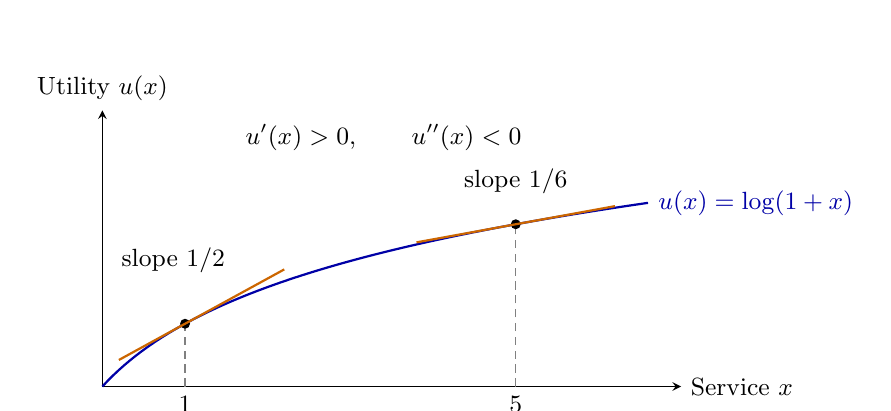
\begin{tikzpicture}[x=1.05cm,y=1.15cm,>=stealth,font=\small]
 \draw[->] (0,0) -- (7,0) node[right] {Service $x$};
 \draw[->] (0,0) -- (0,3.05) node[above] {Utility $u(x)$};
 \draw[thick,blue!65!black,domain=0:6.6,samples=100]
   plot (\x,{ln(1+\x)}) node[right] {$u(x)=\log(1+x)$};
 \draw[densely dashed,gray] (1,0) -- (1,{ln(2)});
 \draw[densely dashed,gray] (5,0) -- (5,{ln(6)});
 \fill (1,{ln(2)}) circle (1.8pt);
 \fill (5,{ln(6)}) circle (1.8pt);
 \draw[thick,orange!80!black,domain=0.2:2.2]
   plot (\x,{ln(2)+(\x-1)/2});
 \draw[thick,orange!80!black,domain=3.8:6.2]
   plot (\x,{ln(6)+(\x-5)/6});
 \node[above left] at (1.6,1.15) {slope $1/2$};
 \node[above] at (5,2.02) {slope $1/6$};
 \node[below] at (1,0) {$1$};
 \node[below] at (5,0) {$5$};
 \node at (3.4,2.75) {$u'(x)>0,\qquad u''(x)<0$};
\end{tikzpicture}
\caption{Increasing, strictly concave utility: the same extra service has a
smaller marginal benefit at a higher service level.}
\label{fig:utility}
\end{figure}

\paragraph{Why a transfer increases the sum of utilities.}
Suppose $0<a<b$, and transfer an amount $\delta$ from the better-served
user to the worse-served user, where
\[
0<\delta<\frac{b-a}{2}.
\]
Define the utility along this transfer by
\[
h(t)=u(a+t)+u(b-t),\qquad 0\leq t\leq\frac{b-a}{2}.
\]
Differentiating gives
\[
h'(t)=u'(a+t)-u'(b-t).
\]
For $0\leq t<(b-a)/2$, we have $a+t<b-t$. Since $u'$ is strictly
decreasing, it follows that
\[
u'(a+t)>u'(b-t),\qquad h'(t)>0.
\]
Consequently,
\[
\begin{aligned}
&u(a+\delta)+u(b-\delta)-u(a)-u(b)\\
&\qquad=\int_0^\delta\bigl(u'(a+t)-u'(b-t)\bigr)\,dt>0.
\end{aligned}
\]
The worse-served user gains more utility from each transferred unit than
the better-served user loses. This proves the required strict increase.

Continuing the transfer until
\[
\delta=\frac{b-a}{2}
\]
gives equal service rates:
\[
a+\delta=b-\delta=\frac{a+b}{2}.
\]
For a fixed total amount of service $a+b$, this is the maximum of the sum
of the two identical strictly concave utilities. Equivalently, strict
concavity gives
\[
u(a)+u(b)<2u\!\left(\frac{a+b}{2}\right)
\quad\text{when }a\ne b.
\]

\paragraph{Equal service is not the same as equal resource use.}
The preceding argument holds the sum of the service rates fixed. It does
not account for a difference in the resources needed to deliver those
rates. If both users cost the same per unit of service, a one-for-one
service transfer preserves resource consumption. In this problem,
however, a unit of service to user 2 costs twice as much as a unit to
user 1.

For example, at the logarithmic optimum $(6,3)$, transferring $\delta>0$
units of service from user 1 to user 2 would give $(6-\delta,3+\delta)$.
Its resource consumption is
\[
(6-\delta)+2(3+\delta)=12+\delta>12,
\]
so the transfer is infeasible. A resource-preserving increase of one unit
in user 2's service instead requires a decrease of two units in user 1's
service. Thus the fixed-service-sum argument cannot simply be applied
to the resource boundary.

Indeed, $u(x)=\log x$ is strictly increasing and strictly concave, but its
sum is maximized at $(6,3)$, not at equal service rates. The equal-service
allocation on the resource boundary is $(4,4)$, and
\[
\log 6+\log 3=\log 18>\log 16=2\log 4.
\]
Strict concavity favors balancing marginal gains subject to feasibility;
it does not, by itself, require equal service rates under unequal costs.

\subsection*{(c)}

\paragraph{The three optimal allocations.}
For total service, the constraint implies
\[
x_1+x_2=(x_1+2x_2)-x_2\leq 12-x_2\leq 12.
\]
Equality requires $x_2=0$ and $x_1=12$. Therefore, the unique maximizer
of total service is
\[
(x_1,x_2)=(12,0).
\]
The objective places all resources with the user who is cheaper to serve.

For logarithmic utility, maximizing $\log x_1+\log x_2$ is equivalent
to maximizing $x_1x_2$ over positive feasible rates. By the arithmetic--
geometric mean inequality,
\[
x_1x_2=\frac{x_1(2x_2)}{2}
\leq\frac{1}{2}\left(\frac{x_1+2x_2}{2}\right)^2
\leq 18.
\]
Equality holds precisely when $x_1=2x_2$ and $x_1+2x_2=12$. Hence,
\[
(x_1,x_2)=(6,3)
\]
is the unique logarithmic-utility maximizer.

For minimum service, put $m=\min\{x_1,x_2\}$. Both rates are at least
$m$, so
\[
3m\leq x_1+2x_2\leq 12,\qquad m\leq 4.
\]
The bound is attained at $(4,4)$. Moreover, attaining $m=4$ requires both
rates to be at least $4$, and the resource constraint then forces both
to equal $4$. The unique optimum is therefore
\[
(x_1,x_2)=(4,4).
\]

The first objective maximizes total service, even at the cost of giving
one user no service. The third maximizes the worst-served user's rate and,
in this particular feasible set, produces equal service. The logarithmic
objective produces neither of those allocations. Its principle is
\emph{proportional fairness}, rather than maximum total service or absolute
equality of service.

\paragraph{The proportional-fairness inequality.}
Let $C\subseteq\mathbb{R}_{>0}^{n}$ be convex, and suppose that
$\mathbf{x}^{\star}$ maximizes
\[
W(\mathbf{x})=\sum_{i=1}^{n}\log x_i
\]
over $C$. Fix any $\mathbf{y}\in C$. Convexity allows us to move along
the line segment from $\mathbf{x}^{\star}$ to $\mathbf{y}$ while staying
feasible:
\[
\mathbf{x}(t)=\mathbf{x}^{\star}
             +t(\mathbf{y}-\mathbf{x}^{\star})\in C,
\qquad 0\leq t\leq 1.
\]
Define
\[
\phi(t)=W\bigl(\mathbf{x}(t)\bigr)
       =\sum_{i=1}^{n}\log\bigl(x_i^{\star}+t(y_i-x_i^{\star})\bigr).
\]
Optimality implies $\phi(t)\leq\phi(0)$ for every $t\in[0,1]$. Thus,
\[
\phi'_+(0)=\lim_{t\downarrow0}\frac{\phi(t)-\phi(0)}{t}\leq0.
\]
Computing this directional derivative yields
\[
\boxed{\displaystyle
\sum_{i=1}^{n}\frac{y_i-x_i^{\star}}{x_i^{\star}}\leq0.}
\]
Each summand is user $i$'s proportional change in service when moving
from $\mathbf{x}^{\star}$ to $\mathbf{y}$. The inequality says that no
feasible alternative can make the sum of these proportional changes
positive: proportional gains must be offset by proportional losses.
It does not say that every individual user must lose. This is the
proportional-fairness criterion.

\paragraph{Weighted logarithmic utility.}
For $W(x_1,x_2)=2\log x_1+\log x_2$, maximizing utility is equivalent
to maximizing $x_1^2x_2$. For the arithmetic--geometric mean inequality, split $x_1$ into two equal terms:
\[
\begin{aligned}
x_1^2x_2
&=2\left(\frac{x_1}{2}\right)
     \left(\frac{x_1}{2}\right)(2x_2)\\
&\leq 2\left(\frac{x_1/2+x_1/2+2x_2}{3}\right)^3\\
&=2\left(\frac{x_1+2x_2}{3}\right)^3
\leq 2\left(\frac{12}{3}\right)^3=128.
\end{aligned}
\]
Equality requires
\[
\frac{x_1}{2}=\frac{x_1}{2}=2x_2,
\qquad x_1+2x_2=12.
\]
Therefore, $x_1=4x_2$, giving the unique optimum
\[
\boxed{(x_1,x_2)=(8,2).}
\]
The coefficient $2$ gives user 1's utility twice the relative importance
in the aggregate objective. Algebraically, it is as if that utility were
counted twice. It need not mean that there are literally two physical
users of type 1; such an interpretation would require an additional
modeling assumption. The weight specifies the designer's trade-off,
not the service cost, which is already encoded in the constraint.

\subsection*{(d)}

\paragraph{Expected payoffs and expected logarithmic utilities.}
Let $X_A=5$ with certainty, while $X_B$ takes values $1$ and $9$ with
equal probabilities. Their expected payoffs are
\[
\mathbb{E}[X_A]=5,\qquad
\mathbb{E}[X_B]=\frac12\cdot1+\frac12\cdot9=5.
\]
Thus, maximizing expected payoff gives indifference between the options.
Their expected logarithmic utilities are instead
\[
\begin{aligned}
\mathbb{E}[\log X_A]&=\log5,\\
\mathbb{E}[\log X_B]&=\frac12\log1+\frac12\log9=\log3.
\end{aligned}
\]
Since $\log5>\log3$, expected logarithmic utility strictly prefers the
certain payoff, Option A.

The logarithmic certainty equivalent of Option B is the certain amount
$c$ whose utility equals the lottery's expected utility:
\[
\log c=\mathbb{E}[\log X_B]=\log3,
\qquad c=3.
\]
Thus, the lottery is equivalent to a certain payoff of $3$ under
logarithmic utility, even though its expected payoff is $5$.

\paragraph{Jensen's inequality and risk aversion.}
For a concave function $u$, Jensen's inequality states, whenever the
quantities are well defined and finite, that
\[
\mathbb{E}[u(X)]\leq u\bigl(\mathbb{E}[X]\bigr).
\]
The right-hand side is the utility of receiving the expected payoff with
certainty. Hence an expected-utility decision maker with concave utility
weakly prefers that certain payoff to the lottery. For strictly concave
utility and a nonconstant lottery, the inequality is strict.

If $u$ is also strictly increasing and the certainty equivalent satisfies
$u(c)=\mathbb{E}[u(X)]$, then
\[
u(c)\leq u\bigl(\mathbb{E}[X]\bigr)
\quad\Longrightarrow\quad c\leq\mathbb{E}[X].
\]
For logarithmic utility this becomes
\[
c=\exp\bigl(\mathbb{E}[\log X]\bigr)\leq\mathbb{E}[X].
\]
This is the risk-aversion interpretation of concavity: uncertainty lowers
the certainty equivalent relative to the expected payoff.

\paragraph{Why this is different from interpersonal fairness.}
Here there is only one user, and utility is averaged over that user's
possible outcomes in different states of uncertainty. In part (b),
utilities are added across different users receiving a deterministic
allocation. The same diminishing-slope property explains both results,
but the comparisons are different: risk aversion concerns uncertainty
for one person, while fairness concerns the distribution across people.
There is no interpersonal allocation to judge as fair or unfair in the
single-user lottery comparison.

\subsection*{(e)}

\paragraph{Lotteries and the four preference axioms.}
Let the finite outcome set be $\mathcal{X}=\{z_1,\ldots,z_n\}$. A
lottery is a probability vector
\[
p=(p_1,\ldots,p_n),\qquad p_i\geq0,\qquad\sum_{i=1}^{n}p_i=1,
\]
where $p_i$ is the probability of outcome $z_i$. The standard axioms on
preferences over all such lotteries are the following.

\begin{enumerate}
\item \textbf{Completeness.} For any lotteries $p,q$, either $p\succeq q$
or $q\succeq p$, or both. Thus every pair of lotteries can be compared;
when both relations hold, write $p\sim q$.

\item \textbf{Transitivity.} If $p\succeq q$ and $q\succeq r$, then
$p\succeq r$. The preference ordering is internally consistent.

\item \textbf{Continuity.} If $p\succ q\succ r$, there exists
$\alpha\in(0,1)$ such that
\[
q\sim\alpha p+(1-\alpha)r.
\]
An intermediate lottery is indifferent to some probability mixture of
the better and worse lotteries; preferences do not have an unbridgeable
jump between them.

\item \textbf{Independence.} For any lotteries $p,q,r$ and
$\alpha\in(0,1)$,
\[
p\succeq q
\quad\Longleftrightarrow\quad
\alpha p+(1-\alpha)r\succeq\alpha q+(1-\alpha)r.
\]
Mixing each of two lotteries with the same third lottery in the same
proportion does not change their ordering.
\end{enumerate}

\paragraph{Expected-utility representation.}
The von Neumann--Morgenstern theorem states that these axioms characterize
preferences that admit an expected-utility representation. There exists
$u:\mathcal{X}\to\mathbb{R}$ such that, writing
\[
U(p)=\mathbb{E}_p[u(Z)]=\sum_{i=1}^{n}p_i u(z_i),
\]
we have
\[
p\succeq q\quad\Longleftrightarrow\quad U(p)\geq U(q).
\]
The decision maker can therefore be represented as choosing a lottery
with maximal expected utility. Conversely, preferences represented in
this way satisfy the four axioms.

\paragraph{Uniqueness up to positive affine transformations.}
If $u$ represents these lottery preferences, then so does
\[
v(z)=a u(z)+b,\qquad a>0,
\]
since
\[
\mathbb{E}_p[v(Z)]=a\mathbb{E}_p[u(Z)]+b.
\]
The same positive scaling and constant shift apply to every lottery, so
no comparison changes. Moreover, any other expected-utility
representation of the same preferences on all lotteries over
$\mathcal{X}$ is related to $u$ by such a positive affine transformation.

The theorem does not require $u$ to be concave, and does not require it
to be logarithmic. Concavity is an additional property relevant to risk
attitudes when outcomes have a numerical payoff interpretation. Nor does
the theorem determine a fair allocation across several users: it
represents a decision maker's lottery preferences, without selecting the
interpersonal utility scales, weights, or fairness objective of a system
designer.

\paragraph{Why an arbitrary increasing transformation is not enough.}
For deterministic outcomes, a strictly increasing transformation preserves
the ordering of utility values. In particular, $u(x)=x$ and $v(x)=\log x$
both give
\[
9\succ5\succ1.
\]
However, expected utility averages the transformed values over possible
outcomes, and a nonlinear transformation can change comparisons between
these averages.

The lotteries in part (d) show this directly. With $u(x)=x$,
\[
\mathbb{E}[u(X_A)]=5
=\frac12\cdot1+\frac12\cdot9
=\mathbb{E}[u(X_B)],
\]
so $A\sim B$. With $v(x)=\log x$,
\[
\mathbb{E}[v(X_A)]=\log5
>\log3
=\mathbb{E}[v(X_B)],
\]
so $A\succ B$. Thus the deterministic rankings coincide, but the lottery
rankings do not. This is why VNM utility is unique up to positive affine
transformations, rather than arbitrary strictly increasing ones.

\subsection*{(f)}

\paragraph{The reward hypothesis and expected utility.}
The reward hypothesis says that an agent's goal can be expressed as the
maximization of the expected cumulative sum of a scalar reward signal.
For this undiscounted, finite-horizon problem, the objective is
\[
J(\pi)=\mathbb{E}_{\pi}\!\left[\sum_{t=0}^{T-1}R_{t+1}\right].
\]
The modeling task is to choose rewards that quantify the intended goal,
so that maximizing this expectation corresponds to pursuing that goal.

This resembles the VNM representation: an abstract preference is
represented numerically, and choices are evaluated by an expectation.
VNM uses the expected utility of an outcome; in sequential decision
making, an entire trajectory can be treated as the outcome, and its
cumulative reward can serve as its utility. The VNM conclusion is
conditional on its preference axioms, whereas the reward hypothesis is
a claim about representing goals in the reward framework.

An expected-utility representation does not automatically give a
stationary Markov reward on a prescribed state space. Such a reward has
a fixed form $r(s,a,s')$, depending only on the current transition, with
no additional dependence on the past or on an external time index. A
utility assigned to a whole trajectory may depend on history that the
specified state does not retain. Consequently, a trajectory-level utility
need not decompose into stationary Markov rewards on that original state
space. Additional state information may be necessary.

\paragraph{Fairness at each time versus fairness of average service.}
The two objectives are
\[
J_{\mathrm{instant}}(\pi)
=\mathbb{E}_{\pi}\!\left[
\sum_{t=0}^{T-1}\bigl(\log X_1(t)+\log X_2(t)\bigr)\right]
\]
and
\[
\begin{aligned}
J_{\mathrm{average}}(\pi)
&=\mathbb{E}_{\pi}\!\left[\log\overline{X}_1
                         +\log\overline{X}_2\right],\\
\overline{X}_i&=\frac{1}{T}\sum_{t=0}^{T-1}X_i(t).
\end{aligned}
\]
The first applies the utility function at every time step and then sums.
The second first averages each user's service over time and only then
applies utility. Since the logarithm is nonlinear, these operations
cannot generally be interchanged.

For $T=2$, all allocations in the two given schedules are feasible and
use the full resource budget:
\[
6+2\cdot3=12,\qquad 10+2\cdot1=12,\qquad 2+2\cdot5=12.
\]
The schedules are deterministic, so the expectations do not change the
following calculations.

For $\pi_A$, the allocation is $(6,3)$ at both time steps. Therefore,
\[
\begin{aligned}
J_{\mathrm{instant}}(\pi_A)
&=2(\log6+\log3)\\
&=2\log18=\log324.
\end{aligned}
\]
Its average service rates are
\[
\overline{X}_1=\frac{6+6}{2}=6,
\qquad
\overline{X}_2=\frac{3+3}{2}=3,
\]
so
\[
J_{\mathrm{average}}(\pi_A)=\log6+\log3=\log18.
\]

For $\pi_B$, the allocations are $(10,1)$ and $(2,5)$. Thus,
\[
\begin{aligned}
J_{\mathrm{instant}}(\pi_B)
&=\log10+\log1+\log2+\log5\\
&=\log100.
\end{aligned}
\]
However, its average service rates are also
\[
\overline{X}_1=\frac{10+2}{2}=6,
\qquad
\overline{X}_2=\frac{1+5}{2}=3.
\]
Consequently,
\[
J_{\mathrm{average}}(\pi_B)=\log6+\log3=\log18.
\]
The instantaneous objective strictly prefers $\pi_A$, because
$\log324>\log100$, while the average-service objective is indifferent
between the schedules. They are therefore not equivalent even as
preference criteria: one gives a strict preference where the other gives
a tie. Under the average-service objective, a user's low service at one
time can be compensated by high service at another time.

\paragraph{A reward that exactly implements average-service utility.}
A direct construction is to give zero reward before the terminal
transition and put the utility of the final averages in the terminal
reward:
\[
R_{t+1}=0\quad(0\leq t<T-1),\qquad
R_T=\log\overline{X}_1+\log\overline{X}_2.
\]
For every realized trajectory,
\[
\sum_{t=0}^{T-1}R_{t+1}
=\log\overline{X}_1+\log\overline{X}_2.
\]
Taking the policy-dependent expectation gives exactly
\[
\mathbb{E}_{\pi}\!\left[\sum_{t=0}^{T-1}R_{t+1}\right]
=J_{\mathrm{average}}(\pi).
\]
Thus the construction works for stochastic policies and trajectories as
well as for the two deterministic examples.

\paragraph{What the state must remember.}
The terminal reward depends on allocations throughout the episode. Rather than the whole history, it is enough
to retain the cumulative service totals
\[
C_i(t)=\sum_{\tau=0}^{t-1}X_i(\tau),\qquad C_i(0)=0,
\qquad i=1,2.
\]
They update recursively as
\[
C_i(t+1)=C_i(t)+X_i(t),
\]
and the terminal reward can be written as
\[
R_T=\log\!\left(\frac{C_1(T)}{T}\right)
   +\log\!\left(\frac{C_2(T)}{T}\right).
\]
If the original state is $S_t$, augment it to
\[
\widetilde{S}_t=\bigl(S_t,C_1(t),C_2(t),t\bigr).
\]
The cumulative totals retain exactly the past information required by
this objective, and the time coordinate determines when the terminal
reward is due. On a transition ending at time $T$, the reward reads the
new totals; on every other transition it is zero. This is a fixed rule
on augmented transitions, rather than a rule requiring access to an
unrecorded history.

Provided that $S_t$ already suffices for the Markov transition dynamics
and the allocation mechanism, this augmentation makes the reward Markov.
Including time also allows the finite-horizon reward rule to be expressed
as a stationary function on the augmented state space. The need for these
extra variables illustrates why an expected-utility representation alone
does not supply a stationary Markov reward on an arbitrary original state
space.

\subsection*{(g)}

VNM expected utility represents preferences over uncertain outcomes by
maximizing expected utility, under the four stated axioms. The reward
hypothesis applies a related representation idea to sequential decisions:
a goal is expressed through expected cumulative scalar reward. A policy
induces a distribution over complete trajectories, so a trajectory can
play the role of the uncertain outcome.

For example, if a trajectory $\tau$ is evaluated by
\[
U(\tau)=\log\overline{X}_1(\tau)+\log\overline{X}_2(\tau),
\]
then the terminal-reward construction in part (f) gives
\[
\mathbb{E}_{\pi}[U(\tau)]
=\mathbb{E}_{\pi}\!\left[\sum_{t=0}^{T-1}R_{t+1}\right].
\]
This makes the connection explicit, but it does not mean that VNM
preferences automatically yield local, stationary Markov rewards.
Trajectory utility may require relevant history to be included in the
state, as the cumulative-service variables do here. Neither the theorem
nor the reward hypothesis, by itself, selects which fairness objective
the designer should adopt.

\end{document}
